\documentclass[a4paper,titlepage,11pt]{article}

\usepackage[top=2.54cm, bottom=2.54cm, left=2.54cm, right=2.54cm]{geometry}
\usepackage[utf8x]{inputenc}
\usepackage{hyperref}
\usepackage{graphicx}
\usepackage{fancyhdr}
\usepackage{lastpage}


\pagestyle{fancy}
\fancyhf{}
\renewcommand{\headrulewidth}{0pt}

\begin{document}

\begin{titlepage}
  \begin{center}
    {\scshape \huge Graph Library \par}
    \vspace{1cm}

    {\scshape \LARGE Project \par}
    \vspace{1.5cm}

    {\scshape \Large Complex Network \par}
    \vspace{0.5cm}

    {\Large Alameda \par}
    \vfill

    {\itshape \Large Group 6 \par}
    \vfill

    \begin{tabular}{l l l}
      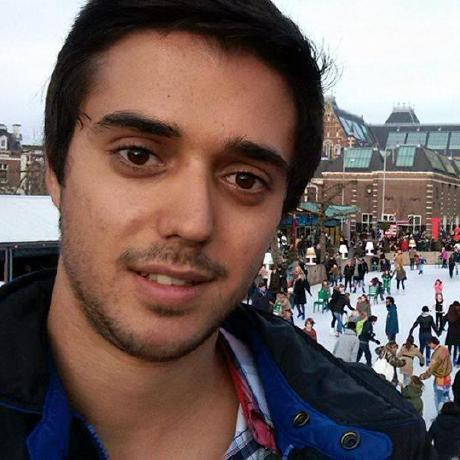
\includegraphics[width=15mm, height=15mm]{img/bernardo.jpeg} & Bernardo Casaleiro & 87827\\
      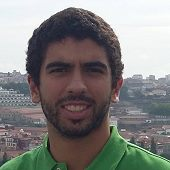
\includegraphics[width=15mm, height=15mm]{img/joao.jpeg} & João Godinho & 87830\\
    \end{tabular}
    \vfill

    {\large \today\par}
  \end{center}
\end{titlepage}







\section{Dataset}
\subsection{Properties}
\subsubsection{Degree Distribution}
\[
  P_k = \frac{N_k}{N} = \frac{1}{N}\sum_{i}{\delta(k_i-k)}
\]
\subsubsection{Clustering Coefficient}
\[
  C_i = \frac{\#\; edges\; among\; neigs}{max\; \# \; edges\; among \; neigs} = \frac{e_i}{k_i(k_i-1)/2}
\]

\[
  \langle C\rangle = \frac{1}{N}\sum_{i}{C_i}
\]
\subsubsection{Average Path Length}
\[
  \langle L\rangle = \frac{1}{N(N-1)}\sum_{ik}{L_{ik}}
\]

\section{Random Graph}
\subsection{Properties}
\subsubsection{Degree Distribution}
\[
  P(k) = {{N-1}\choose{k}} p^{k}(1-p)^{N-1-k}
\]
\subsubsection{Clustering Coefficient}
\[
  C_i = \frac{e_i}{k_i(k_i-1)/2} = p \frac{k_i(k_i-1)/2}{k_i(k_i-1)/2} = p = \frac{\langle k\rangle}{N} 
\]
\subsubsection{Average Path Length}
\[
  APL = \langle L\rangle \simeq \frac{\ln{N}}{\ln{k}}
\]
\end{document}
